\chapter*{Delhi et mariage indien\markboth{Delhi et mariage indien}{}}
\section*{19 décembre 2015}

Je suis invité à côté de Delhi par des amis, Isabelle et Vijay dont le frère va se marier. 

Une journée de visite de la capitale indienne, plongée en permanence dans un brouillard de pollution. 
\begin{center} 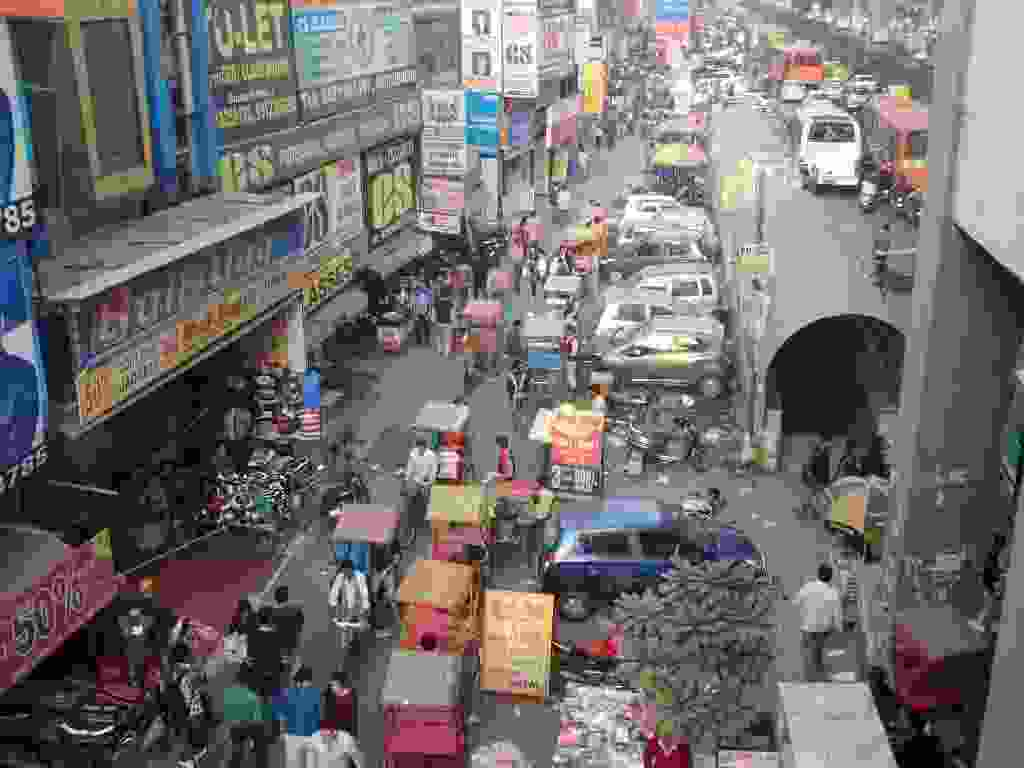
\includegraphics[width=\mywidth]{../wp-content/uploads/2015/12/wpid-oi0005542-1024x768.jpg} \end{center}
\vspace{-\topsep}
\pagebreak

Place Connaugh.
\begin{center} 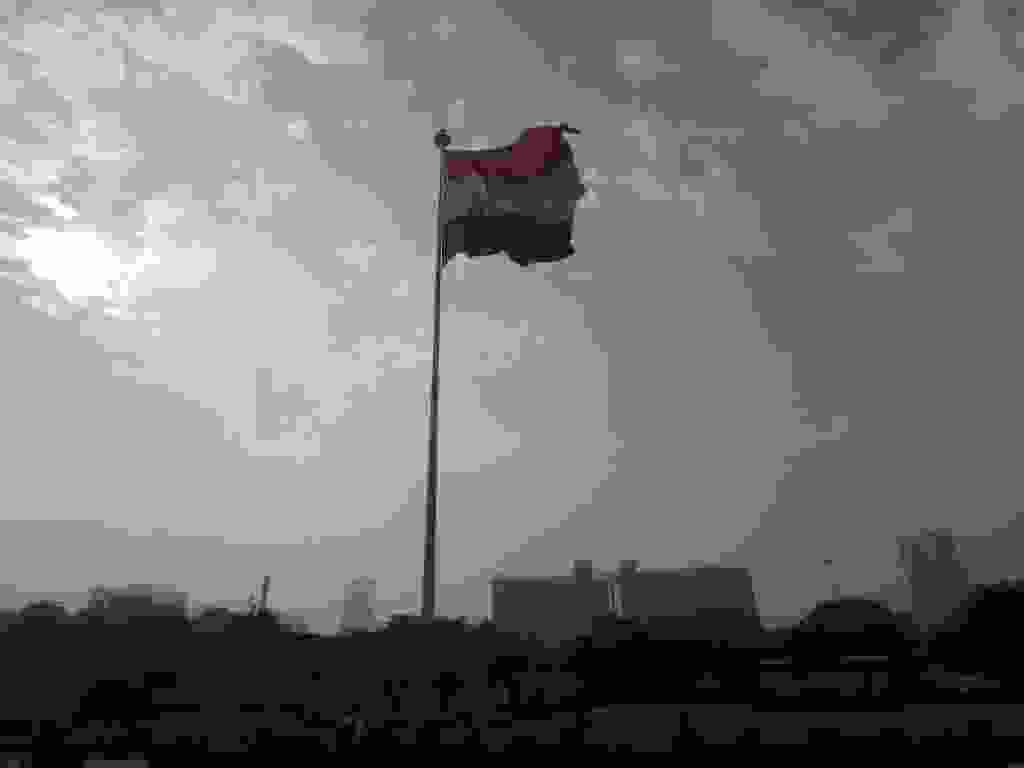
\includegraphics[width=\mywidth]{../wp-content/uploads/2015/12/wpid-oi0005932-1024x768.jpg} \end{center}
\begin{center} 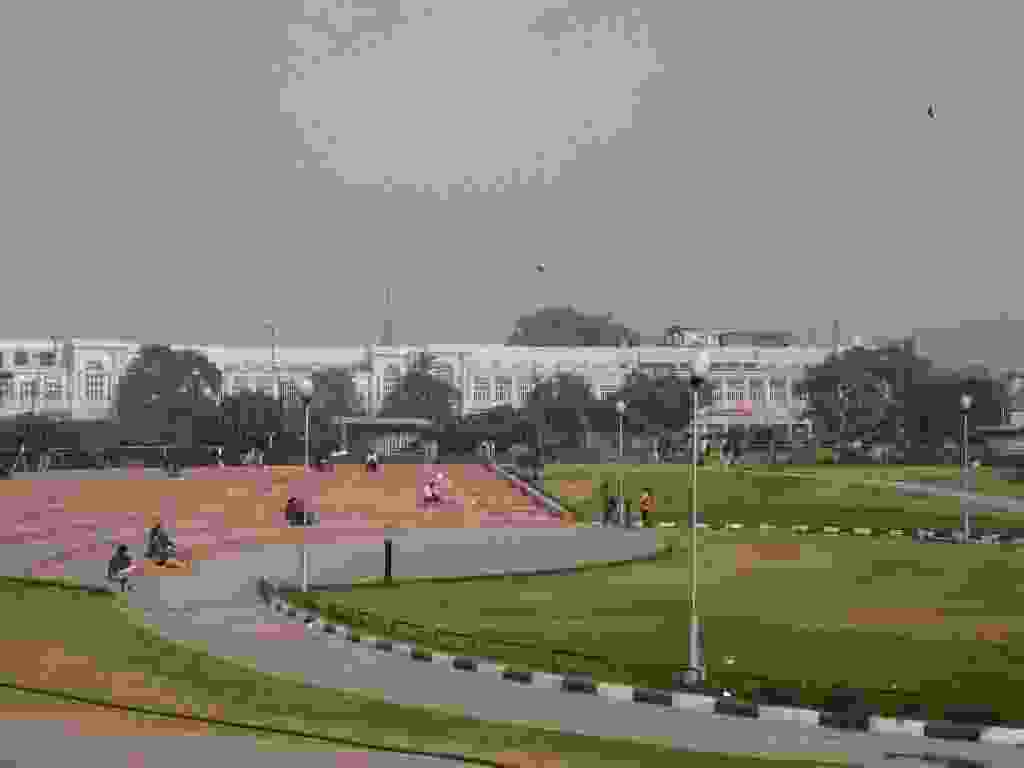
\includegraphics[width=\mywidth]{../wp-content/uploads/2015/12/wpid-oi0005942-1024x768.jpg} \end{center}
\vspace{-\topsep}
\vspace{-3.25mm}
\pagebreak

Old Delhi et le Red Fort.
\begin{center} 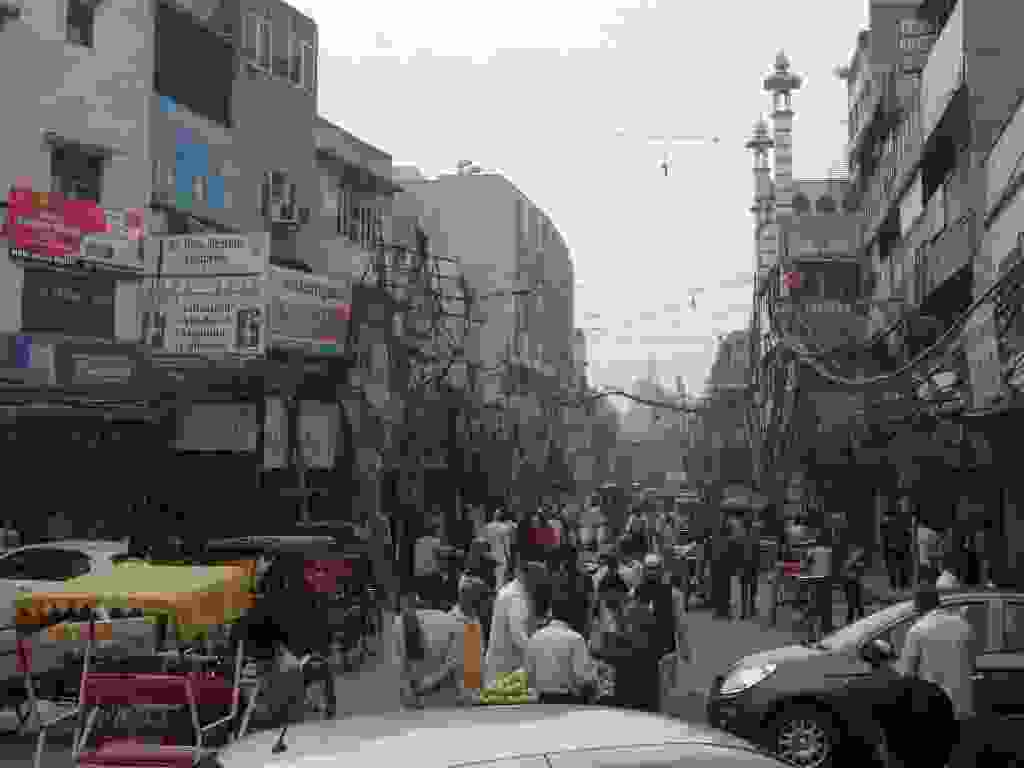
\includegraphics[width=\mywidth]{../wp-content/uploads/2015/12/wpid-oi0006012-1024x768.jpg} \end{center}
\begin{center} 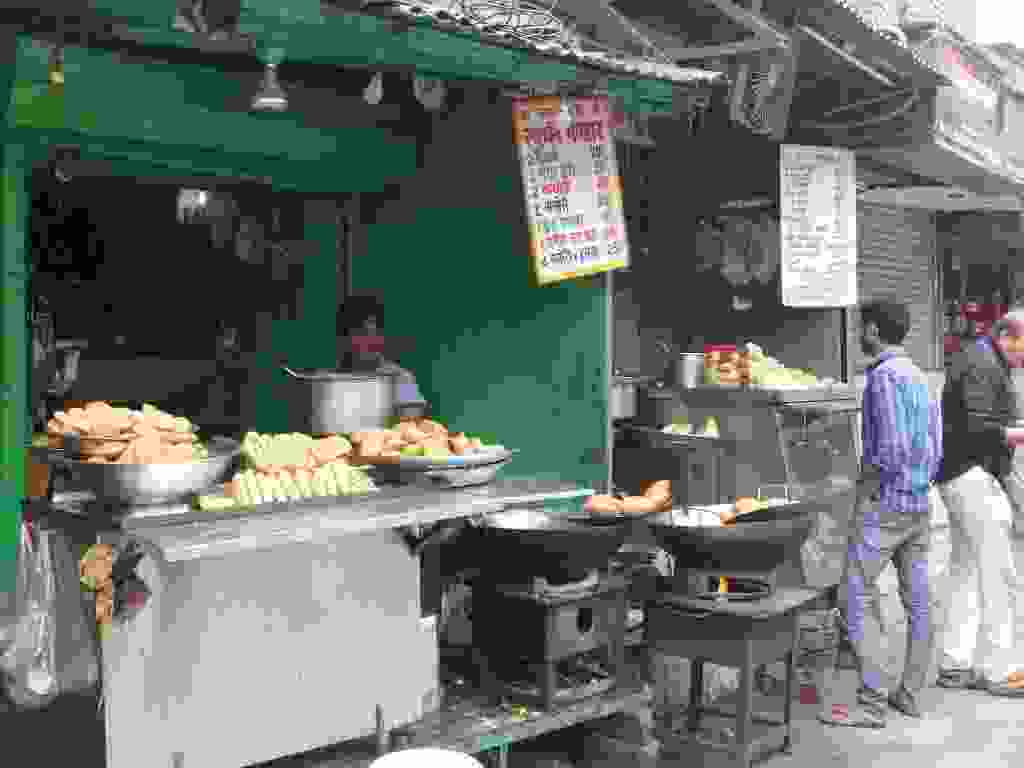
\includegraphics[width=\mywidth]{../wp-content/uploads/2015/12/wpid-oi0006482-1024x768.jpg} \end{center}
\begin{center} 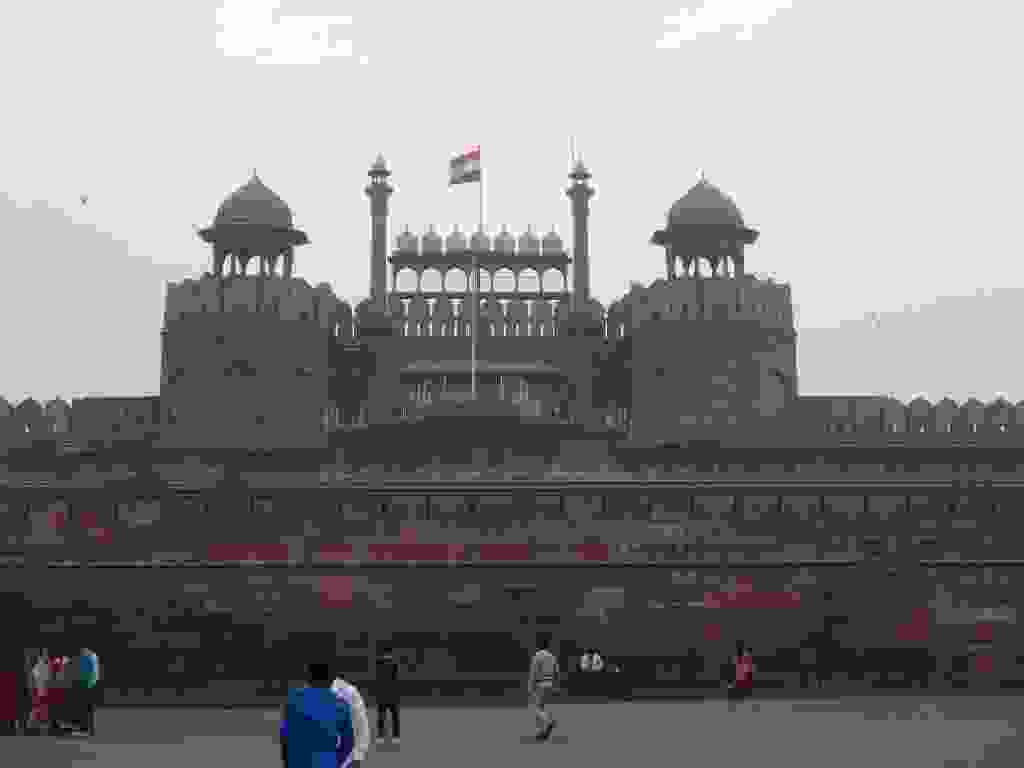
\includegraphics[width=\mywidth]{../wp-content/uploads/2015/12/wpid-oi0006172-1024x768.jpg} \end{center}
\begin{center} 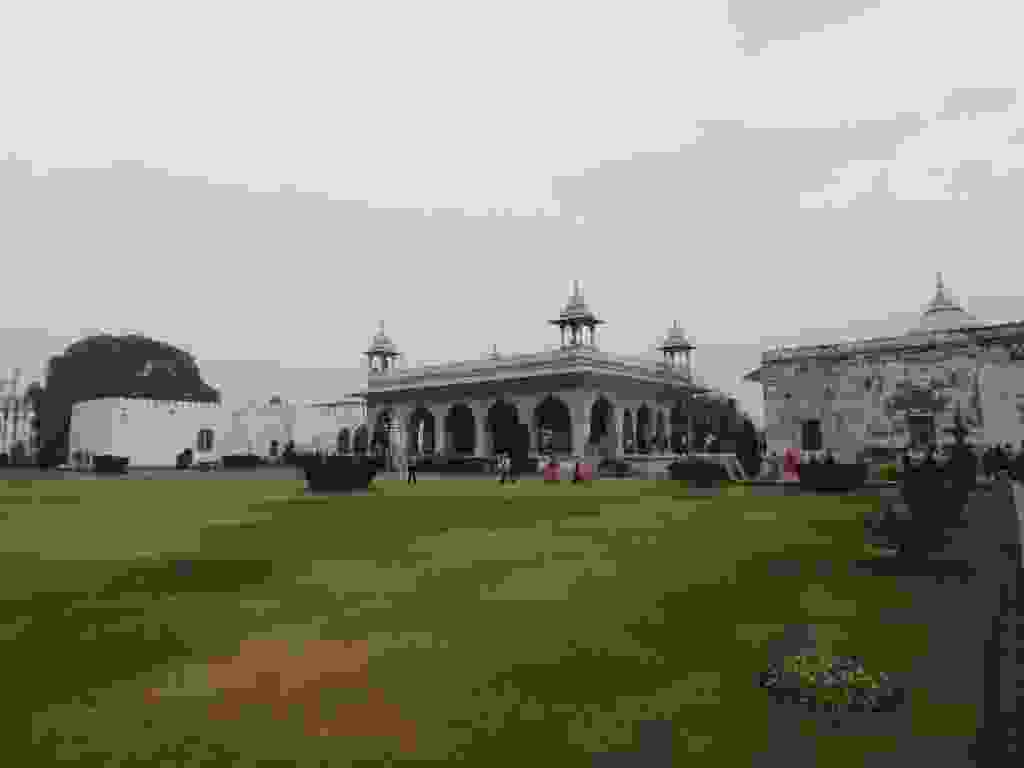
\includegraphics[width=\mywidth]{../wp-content/uploads/2015/12/wpid-oi0006272-1024x768.jpg} \end{center}
\begin{center} 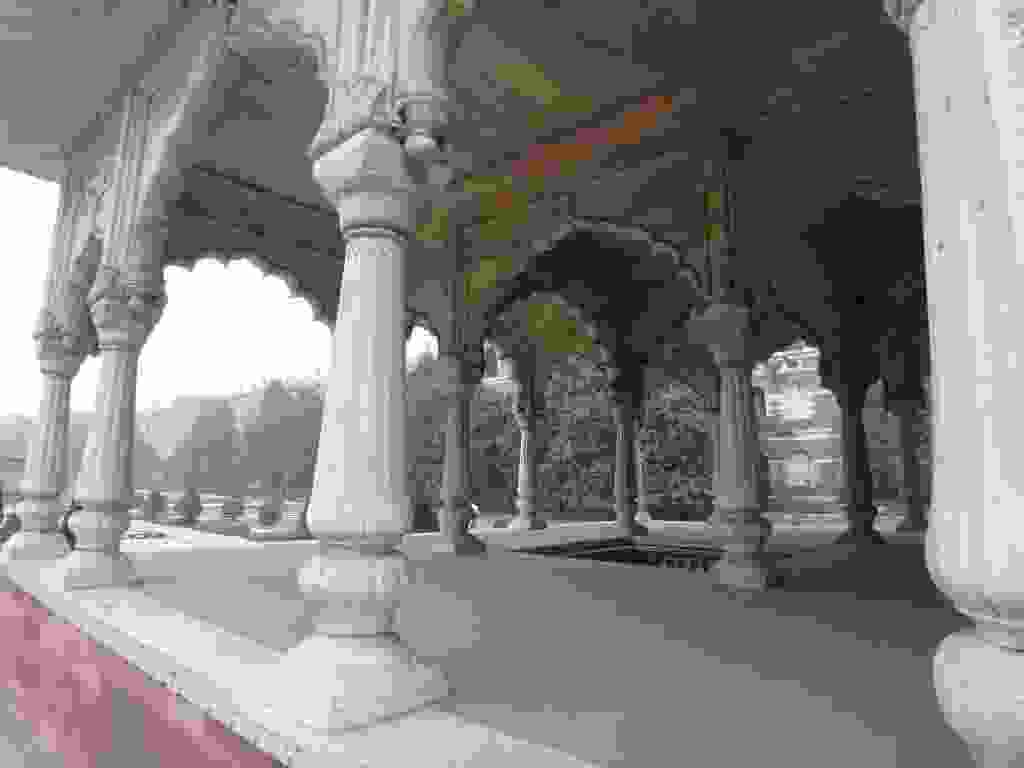
\includegraphics[width=\mywidth]{../wp-content/uploads/2015/12/wpid-oi0006312-1024x768.jpg} \end{center}

Puis je vais à Meerut où a lieu le mariage.

Premier jour, c'est la famille du marié qui invite. 

Je vais voir la préparation du repas, un grand buffet où on peut goûter à plein de spécialités. 
\begin{center} 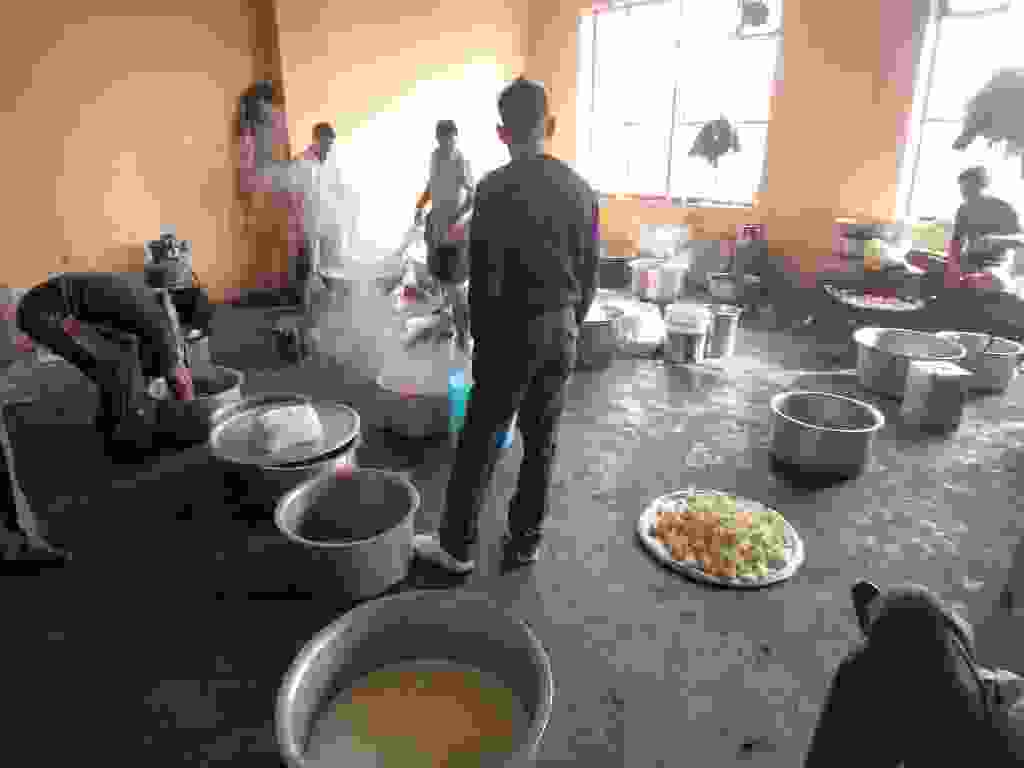
\includegraphics[width=\mywidth]{../wp-content/uploads/2015/12/wpid-oi0006672-1024x768.jpg} \end{center}
\begin{center} 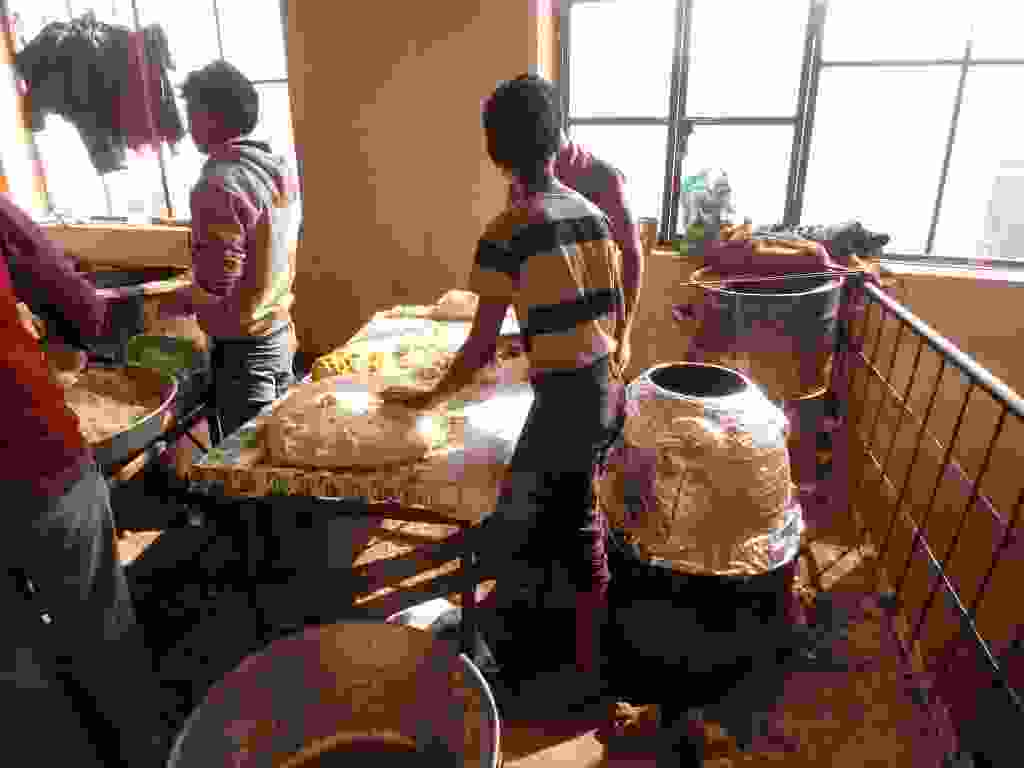
\includegraphics[width=\mywidth]{../wp-content/uploads/2015/12/wpid-oi0006752-1024x768.jpg} \end{center}

Petite cérémonie avec les 2 familles mais sans la mariée. 
\begin{center} 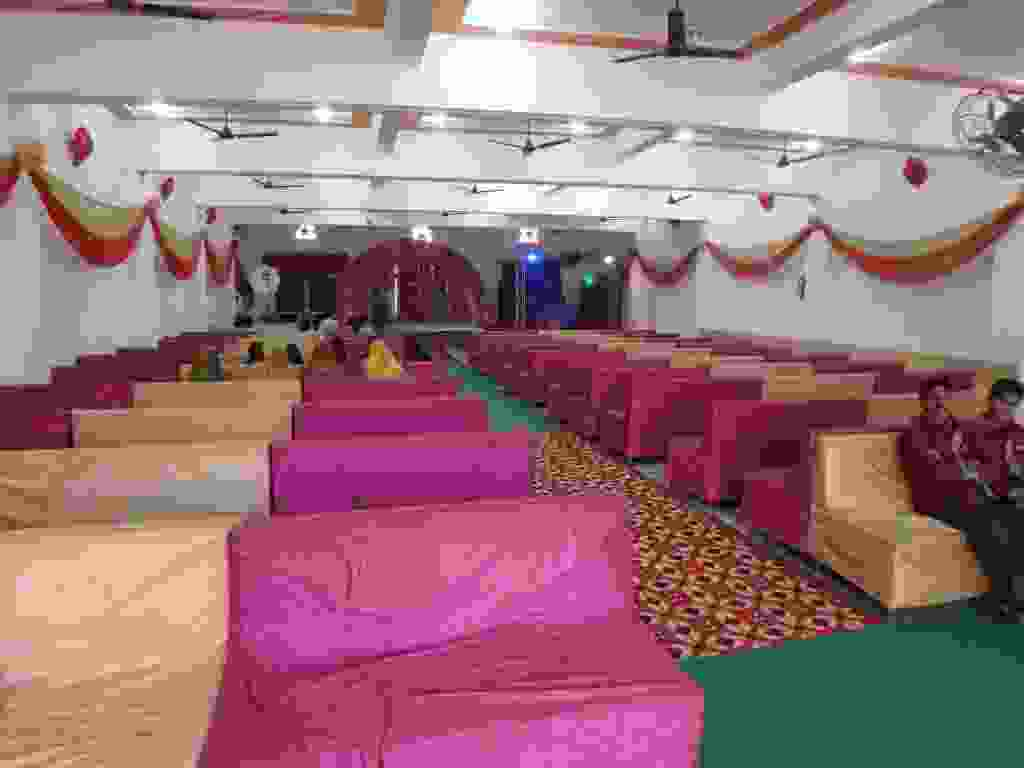
\includegraphics[width=\mywidth]{../wp-content/uploads/2015/12/OI000685-1024x768.jpg} \end{center}
\begin{center} 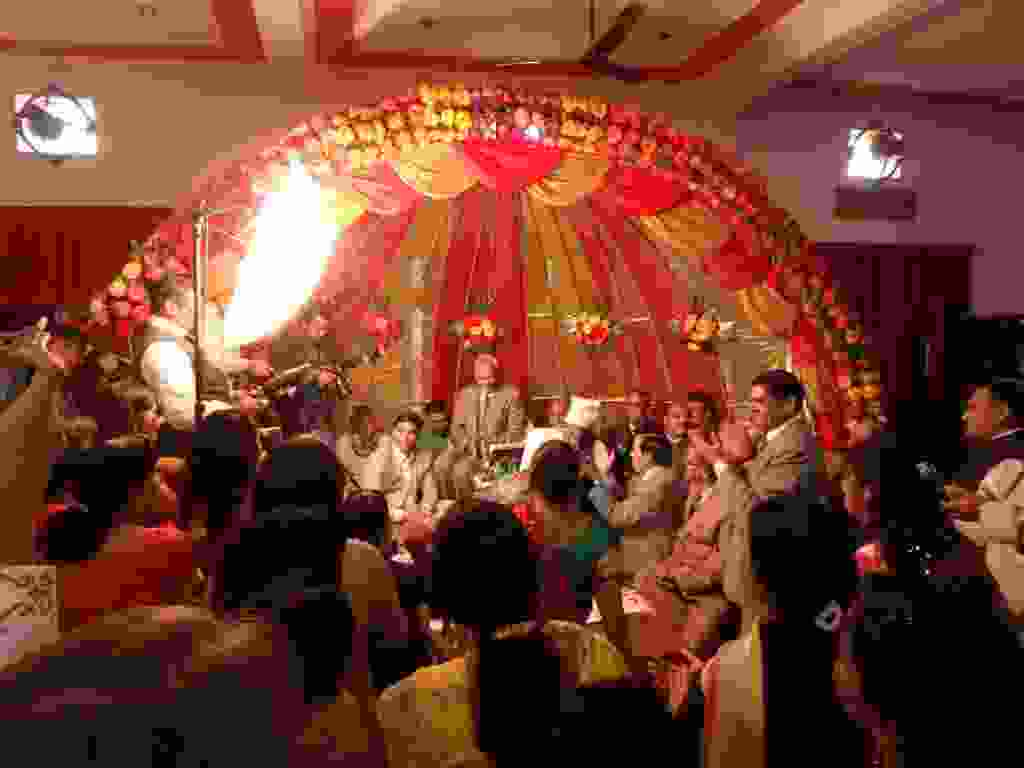
\includegraphics[width=\mywidth]{../wp-content/uploads/2015/12/wpid-oi0007082-1024x768.jpg} \end{center}

Deuxième jour, rituel où le marié est enduit de curcuma, il ne doit plus sortir de la maison jusqu'au mariage. 
\begin{center} 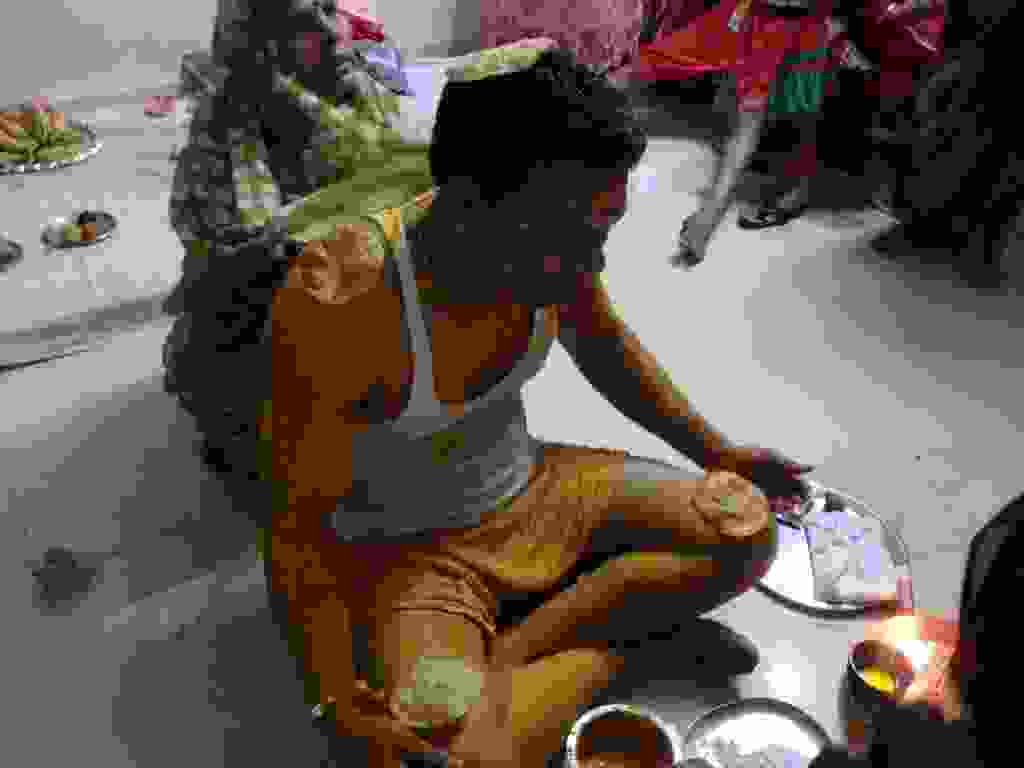
\includegraphics[width=\mywidth]{../wp-content/uploads/2015/12/wpid-oi000732-1024x768.jpg} \end{center}
\vspace{-\topsep}
\pagebreak

Échange de cadeaux dans la famille. 
\begin{center} 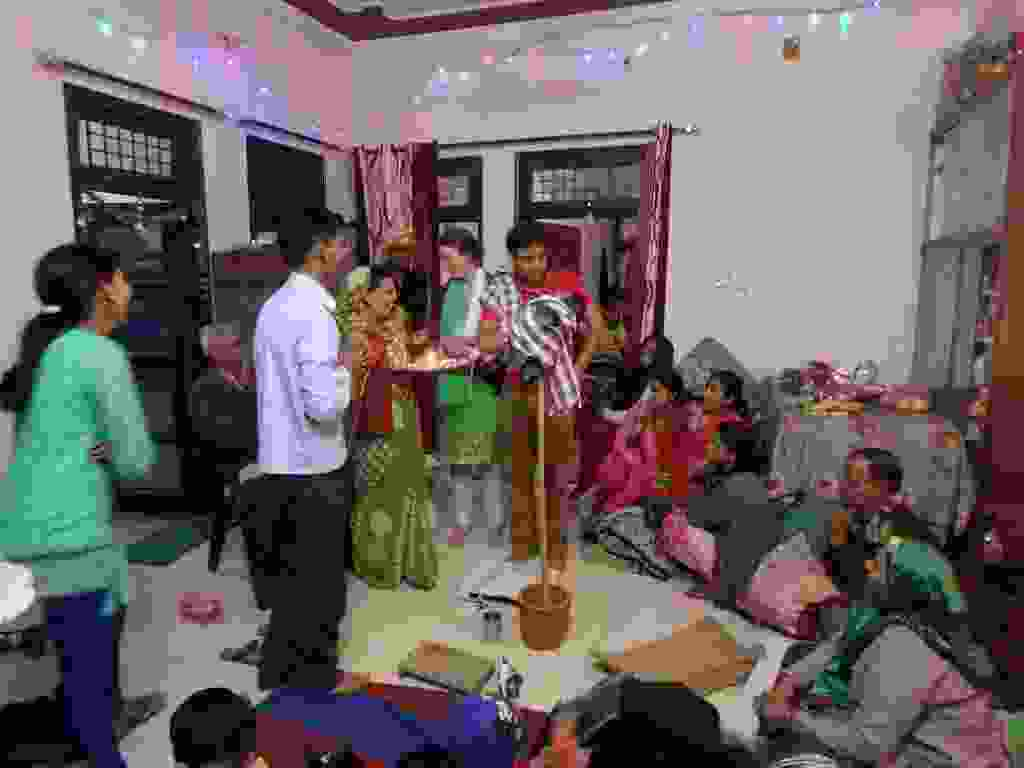
\includegraphics[width=\mywidth]{../wp-content/uploads/2015/12/wpid-oi000739-1024x768.jpg} \end{center}

Troisième jour, le vrai mariage.

Préparation du marié.
\begin{center} 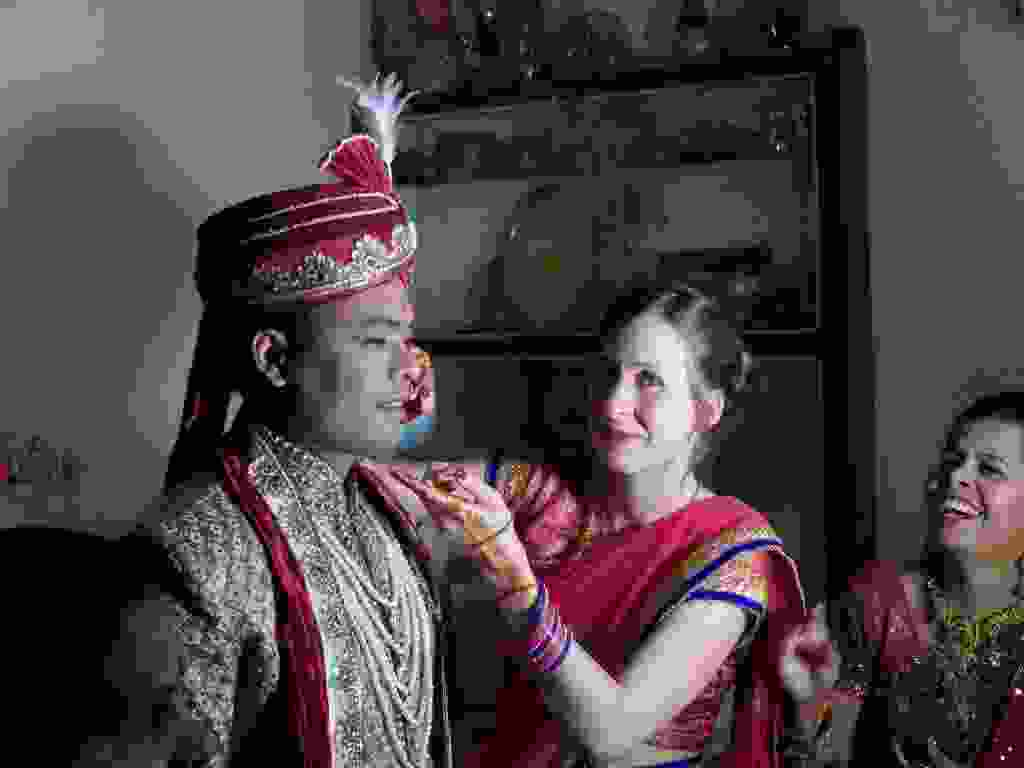
\includegraphics[width=\mywidth]{../wp-content/uploads/2015/12/wpid-oi000752-1024x768.jpg} \end{center}
\vspace{-\topsep}
\pagebreak

Essayage de chapeau, dommage il n'est pas pour moi. 
\begin{center} 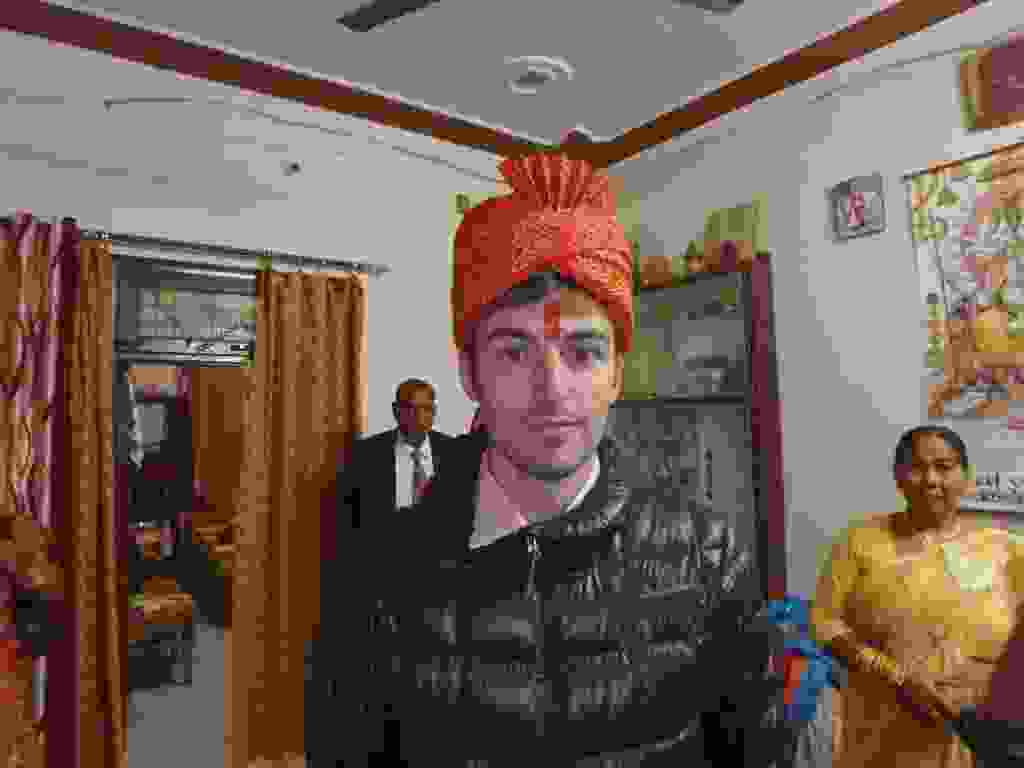
\includegraphics[width=\mywidth]{../wp-content/uploads/2015/12/wpid-oi000745-1024x768.jpg} \end{center}

~

Fanfare devant la maison.
\begin{center} 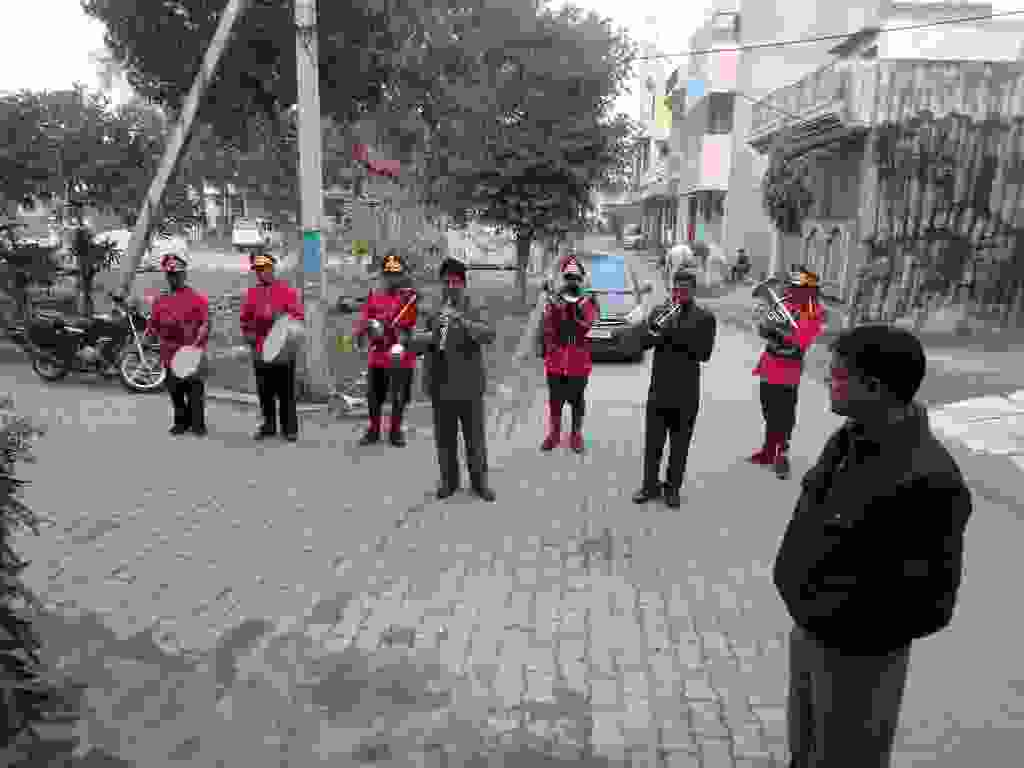
\includegraphics[width=\mywidth]{../wp-content/uploads/2015/12/wpid-oi0007441-1024x768.jpg} \end{center}
\vspace{-\topsep}
\pagebreak

Sortie des 2 frères.
\begin{center} 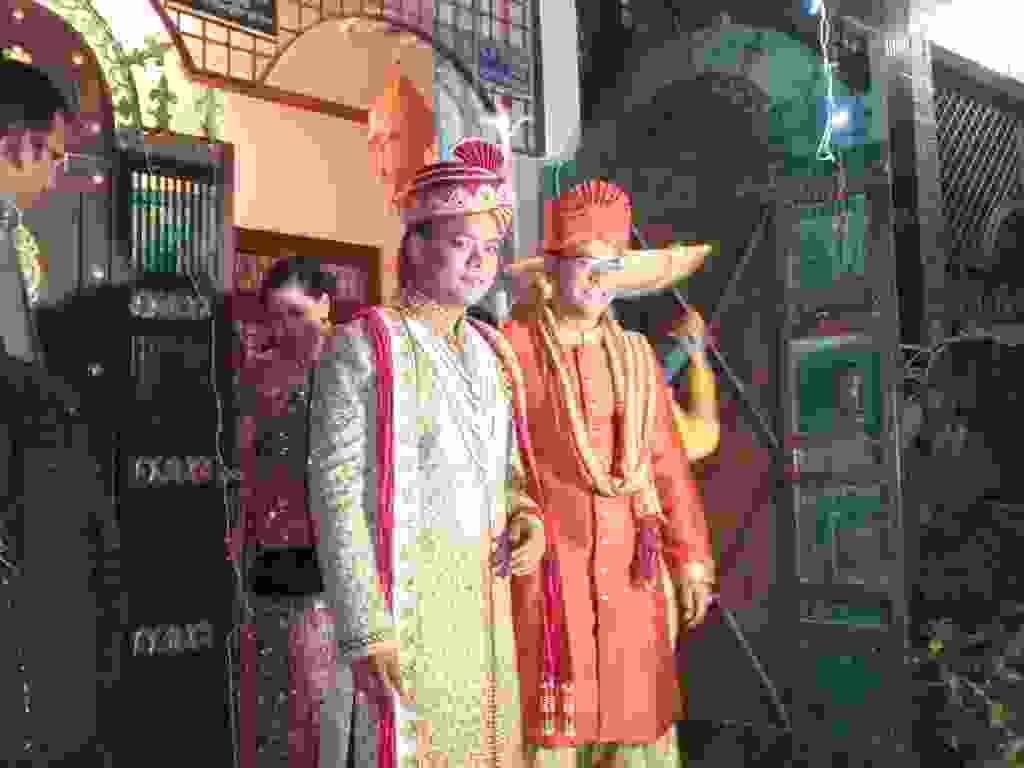
\includegraphics[width=\mywidth]{../wp-content/uploads/2015/12/wpid-oi000754-1024x768.jpg} \end{center}

On accompagne le marié qui va au temple à cheval.

Puis procession avec toute la famille du marié jusqu'au lieu où la famille de la mariée organise le mariage. 
\begin{center} 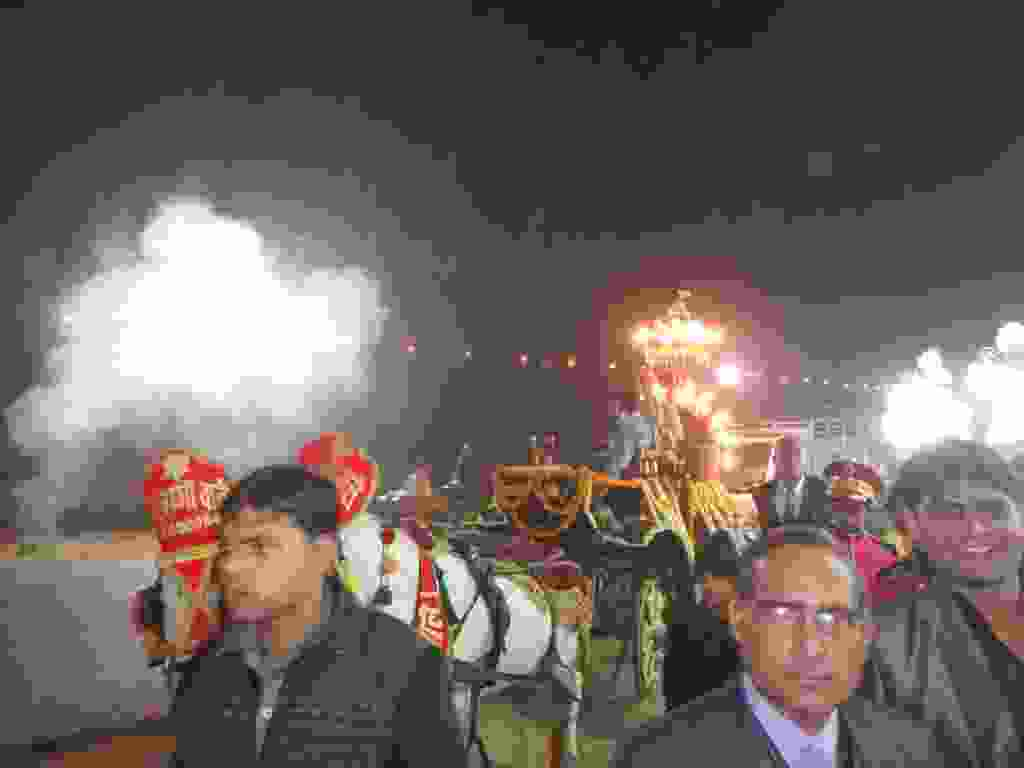
\includegraphics[width=\mywidth]{../wp-content/uploads/2015/12/wpid-oi000760-1024x768.jpg} \end{center}
\vspace{-\topsep}
\pagebreak

~
\vspace{-0.5mm}
\begin{center} 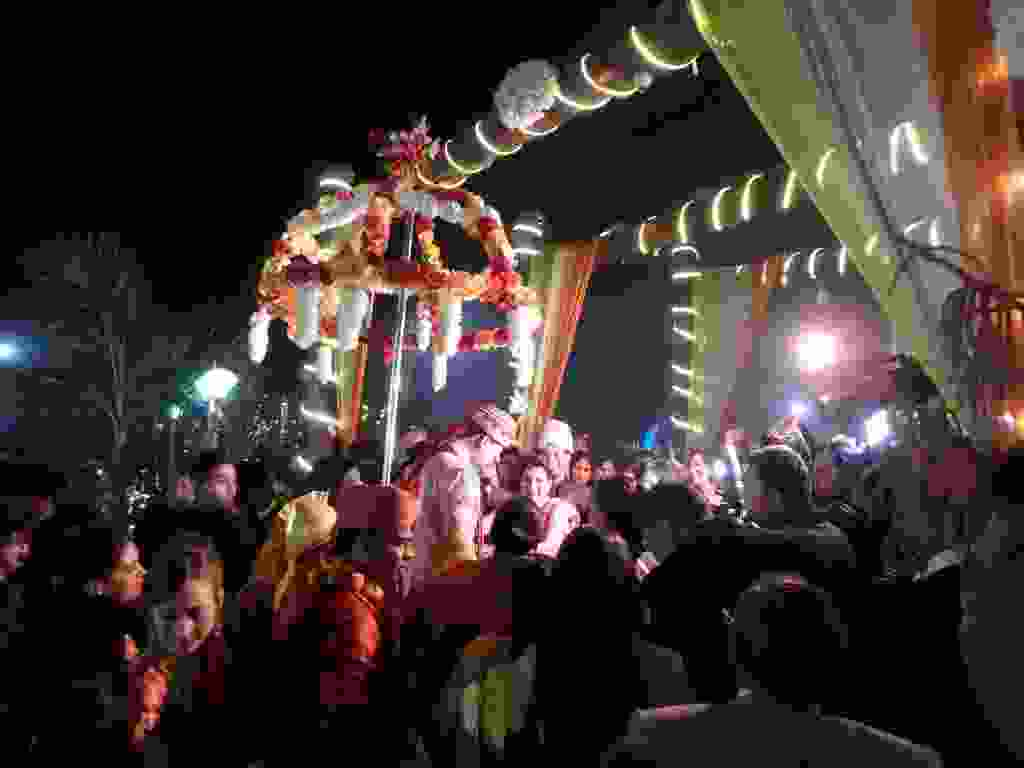
\includegraphics[width=\mywidth]{../wp-content/uploads/2015/12/wpid-oi000762-1024x768.jpg} \end{center}

~

~\\
\begin{center} 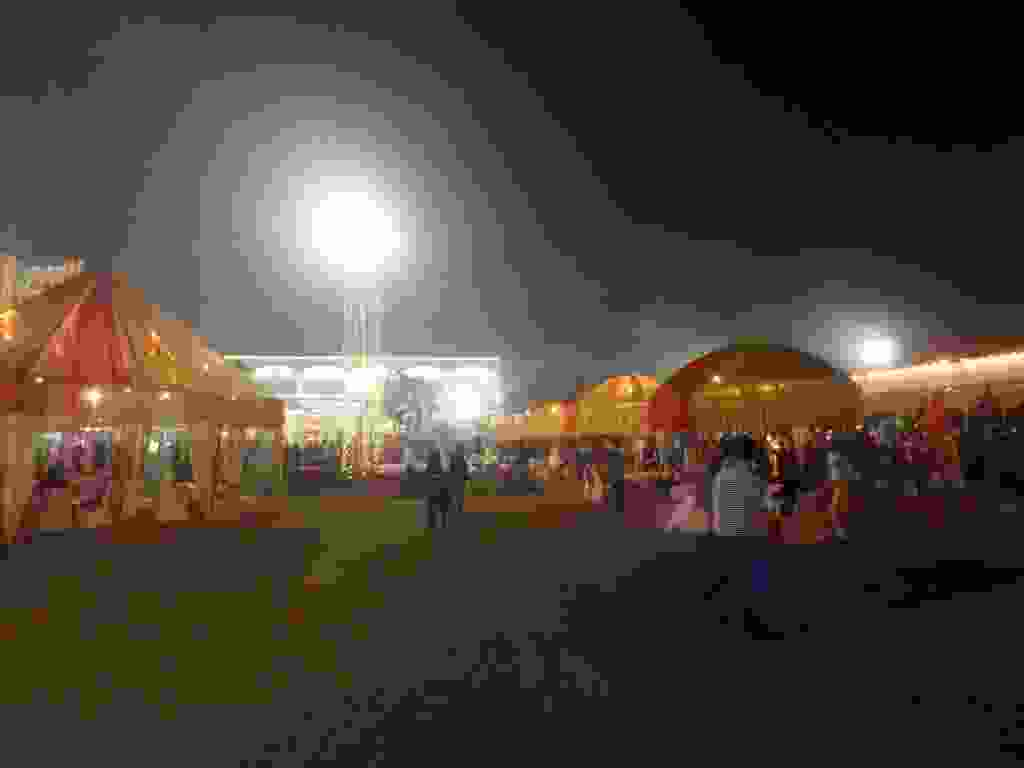
\includegraphics[width=\mywidth]{../wp-content/uploads/2015/12/wpid-oi000763-1024x768.jpg} \end{center}
\vspace{-\topsep}
\pagebreak

Repas encore plus varié que le premier jour.
\begin{center} 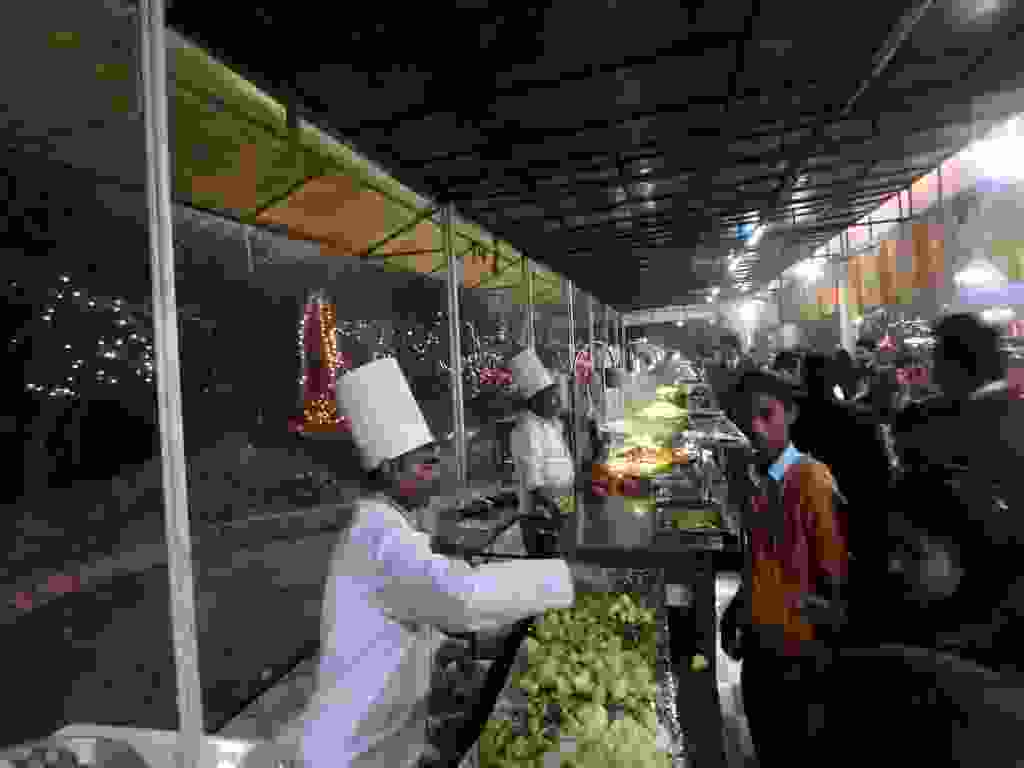
\includegraphics[width=\mywidth]{../wp-content/uploads/2015/12/wpid-oi000766-1024x768.jpg} \end{center}

Séance photo, quasiment tous les invités passent, ça fait quelques centaines de personnes. 
\begin{center} 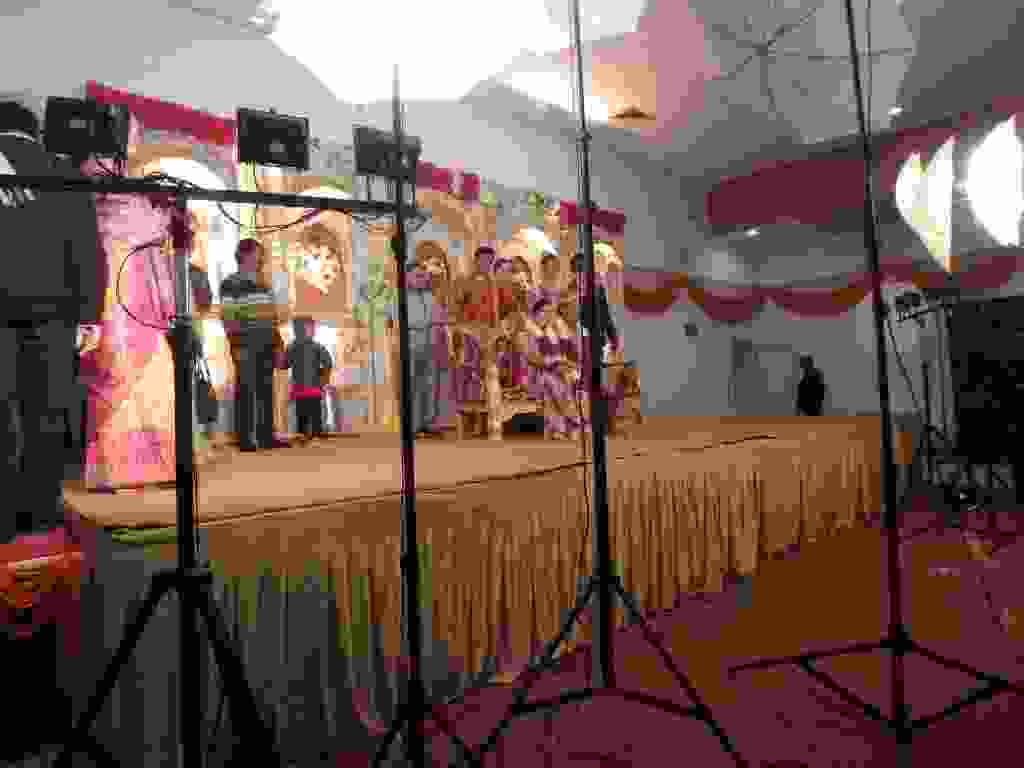
\includegraphics[width=\mywidth]{../wp-content/uploads/2015/12/wpid-oi000774-1024x768.jpg} \end{center}
\vspace{-\topsep}
\pagebreak

Enfin cérémonie autour d'un feu avec le prêtre hindou, entre 2h et 4h du matin. 
\vspace{1mm}
\begin{center} 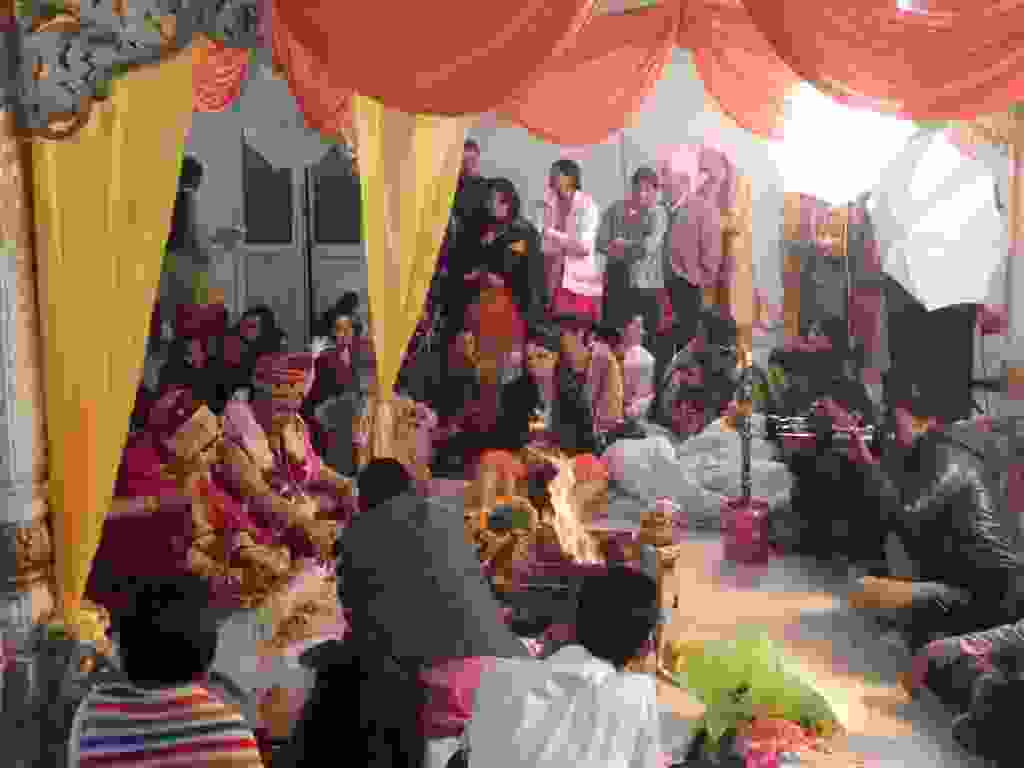
\includegraphics[width=\mywidth]{../wp-content/uploads/2015/12/wpid-oi000783-1024x768.jpg} \end{center}
